\documentclass[8pt,aspectratio=169]{beamer}
\usetheme{Madrid}
\usepackage{graphicx}
\usepackage{booktabs}
\usepackage{adjustbox}
\usepackage{multicol}
\usepackage{amsmath}
\usepackage{amssymb}
\usepackage{tcolorbox}
\usepackage{xcolor}
\usepackage{tikz}
\usetikzlibrary{shapes.geometric, arrows, positioning}
\usepackage{listings}

% Define colors matching the overview presentation
\definecolor{mlblue}{RGB}{31, 119, 180}
\definecolor{mlorange}{RGB}{255, 127, 14}
\definecolor{mlgreen}{RGB}{44, 160, 44}
\definecolor{mlred}{RGB}{214, 39, 40}
\definecolor{mlpurple}{RGB}{148, 103, 189}
\definecolor{mlbrown}{RGB}{140, 86, 75}
\definecolor{mlpink}{RGB}{227, 119, 194}
\definecolor{mlgray}{RGB}{127, 127, 127}
\definecolor{mlyellow}{RGB}{255, 187, 120}
\definecolor{mlcyan}{RGB}{23, 190, 207}

% Remove navigation symbols and add custom footer
\setbeamertemplate{navigation symbols}{}
\setbeamertemplate{footline}{
  \leavevmode%
  \hbox{%
  \begin{beamercolorbox}[wd=.333333\paperwidth,ht=2.25ex,dp=1ex,center]{author in head/foot}%
    \usebeamerfont{author in head/foot}Part \insertpartnumber/4
  \end{beamercolorbox}%
  \begin{beamercolorbox}[wd=.333333\paperwidth,ht=2.25ex,dp=1ex,center]{title in head/foot}%
    \usebeamerfont{title in head/foot}Week 2: Deep Empathy
  \end{beamercolorbox}%
  \begin{beamercolorbox}[wd=.333333\paperwidth,ht=2.25ex,dp=1ex,right]{date in head/foot}%
    \usebeamerfont{date in head/foot}Slide \insertframenumber{} of \inserttotalframenumber\hspace*{2ex} 
  \end{beamercolorbox}}%
  \vskip0pt%
}

% Code listing settings for syntax highlighting
\lstset{
    language=Python,
    basicstyle=\small\ttfamily,
    numbers=left,
    numberstyle=\tiny\color{gray},
    stepnumber=1,
    numbersep=5pt,
    backgroundcolor=\color{gray!5},
    showspaces=false,
    showstringspaces=false,
    showtabs=false,
    frame=single,
    rulecolor=\color{gray!30},
    tabsize=2,
    captionpos=b,
    breaklines=true,
    breakatwhitespace=false,
    keywordstyle=\color{mlblue},
    commentstyle=\color{mlgreen},
    stringstyle=\color{mlorange}
}

\title{\Large\textbf{Machine Learning for Smarter Innovation}\\
\vspace{0.5em}
\Large Week 2: Clustering for Deep Empathy}
\subtitle{Discovering Hidden User Segments at Scale}
\author{BSc Course in AI-Enhanced Innovation}
\date{}

\begin{document}

% Title slide
\begin{frame}
\titlepage
\end{frame}

% Slide 1: Opening Power Chart - Live Clustering Evolution
\begin{frame}
\frametitle{\Large Watch 10,000 Users Organize Themselves}
\framesubtitle{K-Means Evolution: From Chaos to Clarity}

\begin{center}
\includegraphics[width=0.95\textwidth]{charts/clustering_evolution.pdf}
\end{center}

\vspace{-0.2cm}
\begin{tcolorbox}[colback=mlpurple!10, colframe=mlpurple!50]
\centering
\normalsize\textbf{What if users could tell us their natural groups without asking?}
\end{tcolorbox}
\end{frame}

% PART 1: FOUNDATIONS
\part{Why Clustering for Empathy?}

% Section Divider for Part 1
\begin{frame}
\frametitle{\Large Part 1: Foundations}
\framesubtitle{Why Clustering for Deep User Understanding}

\begin{center}
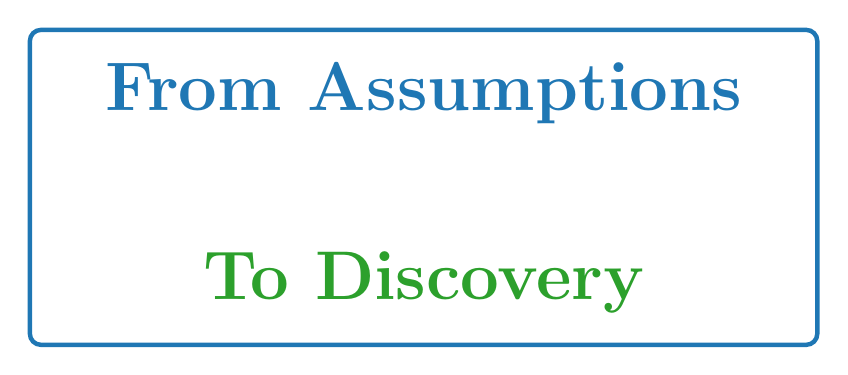
\begin{tikzpicture}[scale=1.2]
\node[draw, ultra thick, mlblue, minimum width=10cm, minimum height=4cm, rounded corners] (box) at (0,0) {};
\node[font=\Huge\bfseries, mlblue] at (0,1) {From Assumptions};
\node[font=\Huge\bfseries, mlgreen] at (0,-1) {To Discovery};
\end{tikzpicture}
\end{center}

\vspace{0.5cm}
\begin{center}
\Large\textit{``One size fits all'' actually fits no one well}
\end{center}
\end{frame}

% Slide 2: The User Understanding Challenge
\begin{frame}
\frametitle{\Large The User Understanding Challenge}
\framesubtitle{Why ``Average User'' Thinking Fails}

\begin{columns}[T]
\begin{column}{0.55\textwidth}
\begin{tcolorbox}[colback=mlred!10, colframe=mlred!50, title=The Problem]
\normalsize
\textbf{Traditional Approach Failures:}
\begin{itemize}
\item Design for ``average user'' → satisfies no one
\item Manual personas → based on assumptions
\item Small sample surveys → miss edge cases
\item Demographics only → ignore behavior patterns
\item Static segments → miss evolution
\end{itemize}
\end{tcolorbox}

\vspace{0.3cm}
\begin{tcolorbox}[colback=mlgreen!10, colframe=mlgreen!50, title=The Opportunity]
\normalsize
\textbf{What if we could:}
\begin{itemize}
\item Find natural user groups automatically?
\item Base segments on actual behavior?
\item Discover unexpected patterns?
\item Track segment evolution?
\end{itemize}
\end{tcolorbox}
\end{column}

\begin{column}{0.43\textwidth}
\begin{center}
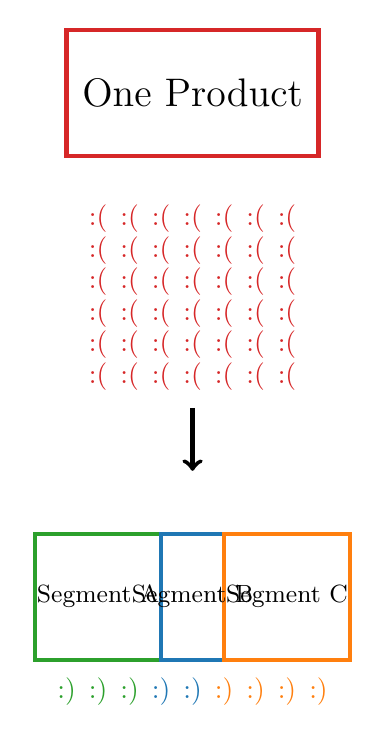
\begin{tikzpicture}[scale=0.8]
% Failed one-size-fits-all visualization
\draw[ultra thick, mlred] (0,4) rectangle (4,6);
\node at (2,5) {\Large One Product};

% Many unhappy users
\foreach \x in {0.5,1,1.5,2,2.5,3,3.5} {
    \foreach \y in {0.5,1,1.5,2,2.5,3} {
        \node[mlred] at (\x,\y) {:(};
    }
}

% Arrow down
\draw[ultra thick, ->] (2,0) -- (2,-1);

% Segmented approach
\draw[ultra thick, mlgreen] (-0.5,-2) rectangle (1.5,-4);
\draw[ultra thick, mlblue] (1.5,-2) rectangle (2.5,-4);
\draw[ultra thick, mlorange] (2.5,-2) rectangle (4.5,-4);

\node at (0.5,-3) {\small Segment A};
\node at (2,-3) {\small Segment B};
\node at (3.5,-3) {\small Segment C};

% Happy users
\foreach \x in {0,0.5,1} {
    \node[mlgreen] at (\x,-4.5) {:)};
}
\foreach \x in {1.5,2} {
    \node[mlblue] at (\x,-4.5) {:)};
}
\foreach \x in {2.5,3,3.5,4} {
    \node[mlorange] at (\x,-4.5) {:)};
}
\end{tikzpicture}
\end{center}
\end{column}
\end{columns}
\end{frame}

% Slide 3: Traditional vs ML Personas
\begin{frame}
\frametitle{\Large Traditional vs ML-Driven Personas}
\framesubtitle{From Assumptions to Data-Driven Discovery}

\begin{columns}[T]
\begin{column}{0.48\textwidth}
\begin{tcolorbox}[colback=mlgray!10, colframe=mlgray!50, title=Traditional Personas]
\normalsize
\textbf{Process:}
\begin{itemize}
\item Interview 10-20 users
\item Create fictional characters
\item Based on demographics
\item Static over time
\end{itemize}

\vspace{0.2cm}
\textbf{Example:}
\begin{itemize}
\item ``Sarah, 35, Marketing Manager''
\item ``Lives in suburbs''
\item ``2 kids, busy lifestyle''
\item ``Values convenience''
\end{itemize}

\vspace{0.2cm}
\textbf{Limitations:}
\begin{itemize}
\item Confirmation bias
\item Small sample size
\item Stereotypes
\item Miss edge cases
\end{itemize}
\end{tcolorbox}
\end{column}

\begin{column}{0.48\textwidth}
\begin{tcolorbox}[colback=mlgreen!10, colframe=mlgreen!50, title=ML-Driven Segments]
\normalsize
\textbf{Process:}
\begin{itemize}
\item Analyze 10,000+ users
\item Find natural groupings
\item Based on behavior patterns
\item Evolve with data
\end{itemize}

\vspace{0.2cm}
\textbf{Discovery:}
\begin{itemize}
\item ``Power Feature Users''
\item ``High engagement, all features''
\item ``Cross demographics''
\item ``Worth 10x average user''
\end{itemize}

\vspace{0.2cm}
\textbf{Advantages:}
\begin{itemize}
\item Data-driven truth
\item Full population
\item Unexpected insights
\item Edge case detection
\end{itemize}
\end{tcolorbox}
\end{column}
\end{columns}

\vspace{0.3cm}
\begin{center}
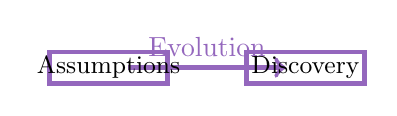
\begin{tikzpicture}
\draw[ultra thick, mlpurple, ->] (0,0) -- (2,0) node[midway, above] {Evolution};
\draw[ultra thick, mlpurple] (-1,-0.2) rectangle (0.5,0.2);
\draw[ultra thick, mlpurple] (1.5,-0.2) rectangle (3,0.2);
\node at (-0.25,0) {\small Assumptions};
\node at (2.25,0) {\small Discovery};
\end{tikzpicture}
\end{center}
\end{frame}

% Slide 4: Types of User Segmentation
\begin{frame}
\frametitle{\Large Types of User Segmentation}
\framesubtitle{Different Lenses for Understanding Users}

\begin{center}
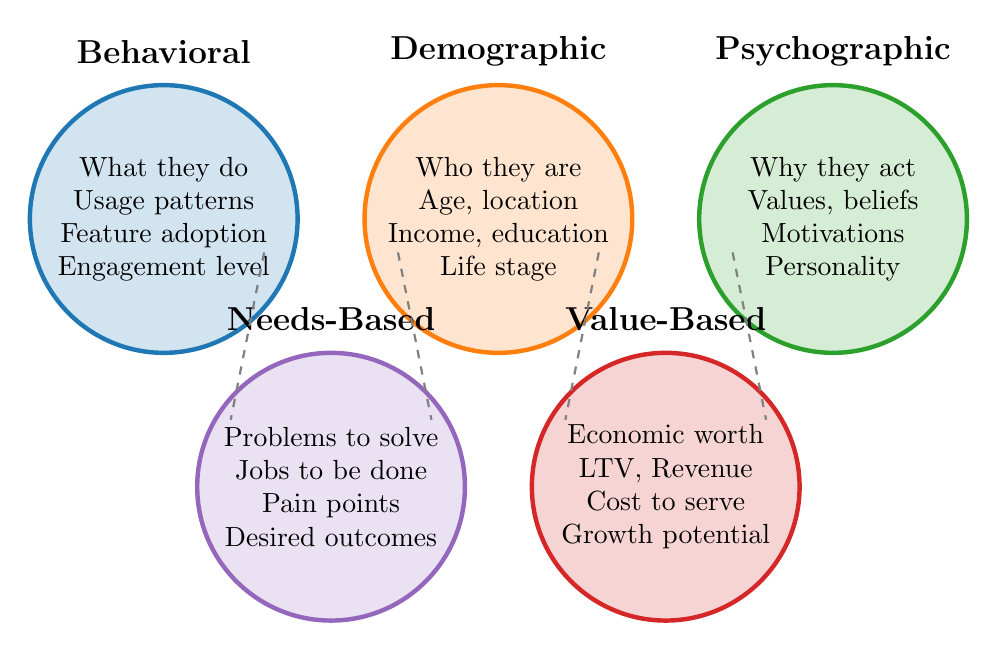
\begin{tikzpicture}[scale=0.85]
% Behavioral
\draw[ultra thick, mlblue, fill=mlblue!20] (0,0) circle (2);
\node[font=\large\bfseries] at (0,2.5) {Behavioral};
\node[align=center] at (0,0) {What they do\\Usage patterns\\Feature adoption\\Engagement level};

% Demographic  
\draw[ultra thick, mlorange, fill=mlorange!20] (5,0) circle (2);
\node[font=\large\bfseries] at (5,2.5) {Demographic};
\node[align=center] at (5,0) {Who they are\\Age, location\\Income, education\\Life stage};

% Psychographic
\draw[ultra thick, mlgreen, fill=mlgreen!20] (10,0) circle (2);
\node[font=\large\bfseries] at (10,2.5) {Psychographic};
\node[align=center] at (10,0) {Why they act\\Values, beliefs\\Motivations\\Personality};

% Needs-based
\draw[ultra thick, mlpurple, fill=mlpurple!20] (2.5,-4) circle (2);
\node[font=\large\bfseries] at (2.5,-1.5) {Needs-Based};
\node[align=center] at (2.5,-4) {Problems to solve\\Jobs to be done\\Pain points\\Desired outcomes};

% Value-based
\draw[ultra thick, mlred, fill=mlred!20] (7.5,-4) circle (2);
\node[font=\large\bfseries] at (7.5,-1.5) {Value-Based};
\node[align=center] at (7.5,-4) {Economic worth\\LTV, Revenue\\Cost to serve\\Growth potential};

% Connections showing overlap
\draw[dashed, thick, gray] (1.5,-0.5) -- (1,-3);
\draw[dashed, thick, gray] (3.5,-0.5) -- (4,-3);
\draw[dashed, thick, gray] (6.5,-0.5) -- (6,-3);
\draw[dashed, thick, gray] (8.5,-0.5) -- (9,-3);
\end{tikzpicture}
\end{center}

\vspace{0.3cm}
\begin{tcolorbox}[colback=mlcyan!10, colframe=mlcyan!50]
\centering
\normalsize\textbf{ML Clustering can combine ALL dimensions simultaneously!}
\end{tcolorbox}
\end{frame}

% PART 2: TECHNICAL DEEP DIVE
\part{The Mathematics of Understanding}

% Section Divider for Part 2
\begin{frame}
\frametitle{\Large Part 2: Technical Deep Dive}
\framesubtitle{The Mathematics Behind User Understanding}

\begin{center}
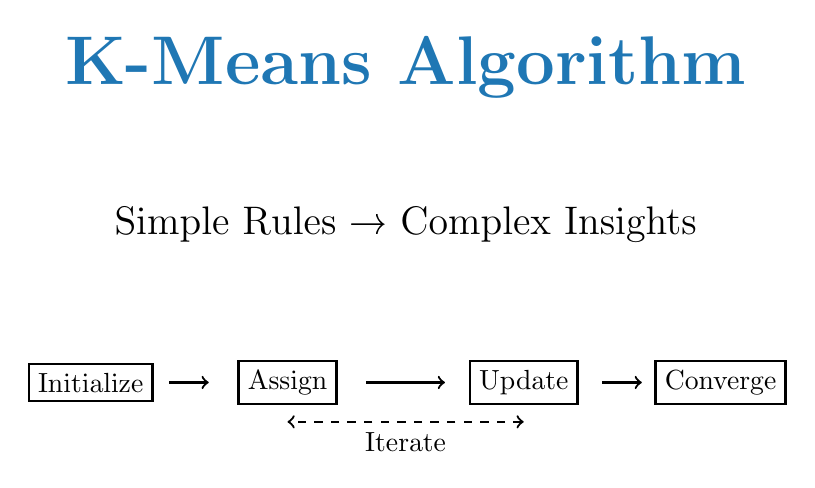
\begin{tikzpicture}[scale=1]
\node[font=\Huge\bfseries, mlblue] at (0,2) {K-Means Algorithm};
\node[font=\Large] at (0,0) {Simple Rules → Complex Insights};

% Algorithm flow
\node[draw, thick] at (-4,-2) {Initialize};
\node[draw, thick] at (-1.5,-2) {Assign};
\node[draw, thick] at (1.5,-2) {Update};
\node[draw, thick] at (4,-2) {Converge};

\draw[thick, ->] (-3,-2) -- (-2.5,-2);
\draw[thick, ->] (-0.5,-2) -- (0.5,-2);
\draw[thick, ->] (2.5,-2) -- (3,-2);
\draw[thick, <->, dashed] (1.5,-2.5) -- (-1.5,-2.5) node[midway, below] {Iterate};
\end{tikzpicture}
\end{center}
\end{frame}

% Slide 5: K-means Algorithm Mechanics
\begin{frame}
\frametitle{\Large K-means Algorithm Mechanics}
\framesubtitle{The Four-Step Dance}

\begin{columns}[T]
\begin{column}{0.48\textwidth}
\textbf{\large The Algorithm:}

\begin{enumerate}
\item \textbf{Initialize:} Choose k random centers
\item \textbf{Assign:} Each point → nearest center
\item \textbf{Update:} Centers move to mean
\item \textbf{Repeat:} Until centers stop moving
\end{enumerate}

\vspace{0.5cm}
\textbf{\large Mathematical Objective:}
$$\min \sum_{i=1}^{n} \sum_{j=1}^{k} w_{ij} ||x_i - \mu_j||^2$$

Where:
\begin{itemize}
\item $x_i$ = data point $i$
\item $\mu_j$ = center of cluster $j$  
\item $w_{ij} = 1$ if $x_i$ belongs to cluster $j$
\end{itemize}
\end{column}

\begin{column}{0.48\textwidth}
\begin{center}
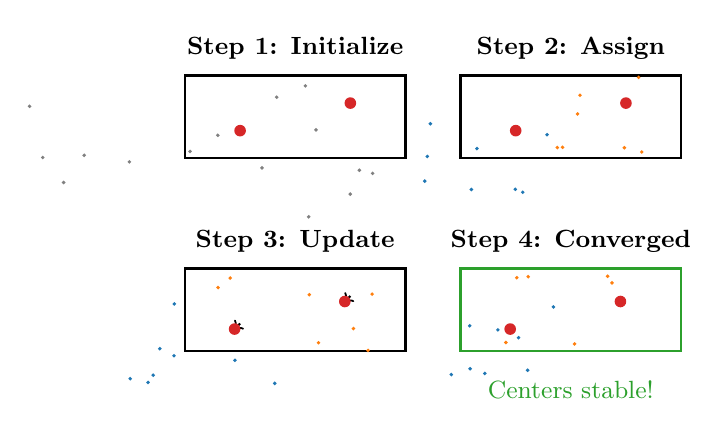
\begin{tikzpicture}[scale=0.7]
% Step 1: Initialize
\node[font=\small\bfseries] at (2,6) {Step 1: Initialize};
\draw[thick] (0,4) rectangle (4,5.5);
\foreach \i in {1,...,15} {
    \fill[gray] (rand*3.5+0.25, rand*1.25+4.125) circle (1pt);
}
\fill[mlred] (1,4.5) circle (3pt);
\fill[mlred] (3,5) circle (3pt);

% Step 2: Assign
\node[font=\small\bfseries] at (7,6) {Step 2: Assign};
\draw[thick] (5,4) rectangle (9,5.5);
\foreach \i in {1,...,8} {
    \fill[mlblue] (rand*1.5+5.25, rand*0.75+4.125) circle (1pt);
}
\foreach \i in {1,...,7} {
    \fill[mlorange] (rand*1.5+7, rand*0.75+4.75) circle (1pt);
}
\fill[mlred] (6,4.5) circle (3pt);
\fill[mlred] (8,5) circle (3pt);

% Step 3: Update
\node[font=\small\bfseries] at (2,2.5) {Step 3: Update};
\draw[thick] (0,0.5) rectangle (4,2);
\foreach \i in {1,...,8} {
    \fill[mlblue] (rand*1.5+0.25, rand*0.75+0.625) circle (1pt);
}
\foreach \i in {1,...,7} {
    \fill[mlorange] (rand*1.5+2, rand*0.75+1.25) circle (1pt);
}
\draw[thick, ->] (1,1) -- (0.9,0.9);
\draw[thick, ->] (3,1.5) -- (2.9,1.4);
\fill[mlred] (0.9,0.9) circle (3pt);
\fill[mlred] (2.9,1.4) circle (3pt);

% Step 4: Converged
\node[font=\small\bfseries] at (7,2.5) {Step 4: Converged};
\draw[thick, mlgreen] (5,0.5) rectangle (9,2);
\foreach \i in {1,...,8} {
    \fill[mlblue] (rand*1.5+5.25, rand*0.75+0.625) circle (1pt);
}
\foreach \i in {1,...,7} {
    \fill[mlorange] (rand*1.5+7, rand*0.75+1.25) circle (1pt);
}
\fill[mlred] (5.9,0.9) circle (3pt);
\fill[mlred] (7.9,1.4) circle (3pt);
\node[mlgreen] at (7,-0.2) {\small Centers stable!};
\end{tikzpicture}
\end{center}
\end{column}
\end{columns}
\end{frame}

% Slide 6: Distance Metrics & Centroids
\begin{frame}
\frametitle{\Large Distance Metrics \& Centroids}
\framesubtitle{How We Measure ``Similar''}

\begin{columns}[T]
\begin{column}{0.33\textwidth}
\begin{tcolorbox}[colback=mlblue!10, colframe=mlblue!50, title=Euclidean]
\centering
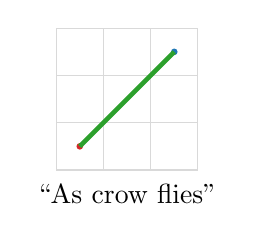
\begin{tikzpicture}[scale=0.6]
\draw[gray!30] (0,0) grid (3,3);
\fill[mlred] (0.5,0.5) circle (2pt);
\fill[mlblue] (2.5,2.5) circle (2pt);
\draw[ultra thick, mlgreen] (0.5,0.5) -- (2.5,2.5);
\node at (1.5,-0.5) {``As crow flies''};
\end{tikzpicture}

$$d = \sqrt{(x_2-x_1)^2 + (y_2-y_1)^2}$$

\small
\textbf{Use when:}
\begin{itemize}
\item Physical distance
\item Continuous features
\item Equal scale
\end{itemize}
\end{tcolorbox}
\end{column}

\begin{column}{0.33\textwidth}
\begin{tcolorbox}[colback=mlorange!10, colframe=mlorange!50, title=Manhattan]
\centering
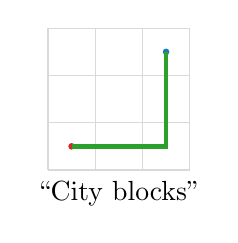
\begin{tikzpicture}[scale=0.6]
\draw[gray!30] (0,0) grid (3,3);
\fill[mlred] (0.5,0.5) circle (2pt);
\fill[mlblue] (2.5,2.5) circle (2pt);
\draw[ultra thick, mlgreen] (0.5,0.5) -- (2.5,0.5) -- (2.5,2.5);
\node at (1.5,-0.5) {``City blocks''};
\end{tikzpicture}

$$d = |x_2-x_1| + |y_2-y_1|$$

\small
\textbf{Use when:}
\begin{itemize}
\item Grid-like data
\item Feature differences
\item Outlier robust
\end{itemize}
\end{tcolorbox}
\end{column}

\begin{column}{0.33\textwidth}
\begin{tcolorbox}[colback=mlgreen!10, colframe=mlgreen!50, title=Cosine]
\centering
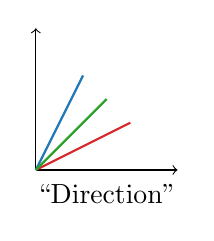
\begin{tikzpicture}[scale=0.6]
\draw[->] (0,0) -- (3,0);
\draw[->] (0,0) -- (0,3);
\draw[thick, mlred] (0,0) -- (2,1);
\draw[thick, mlblue] (0,0) -- (1,2);
\draw[thick, mlgreen] (0,0) -- (1.5,1.5);
\node at (1.5,-0.5) {``Direction''};
\end{tikzpicture}

$$\cos(\theta) = \frac{A \cdot B}{||A|| \cdot ||B||}$$

\small
\textbf{Use when:}
\begin{itemize}
\item Text/documents
\item High dimensions
\item Magnitude varies
\end{itemize}
\end{tcolorbox}
\end{column}
\end{columns}

\vspace{0.5cm}
\begin{center}
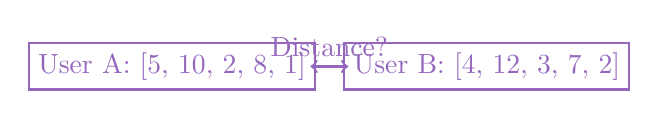
\begin{tikzpicture}[scale=0.8]
\node[draw, thick, mlpurple] at (0,0) {User A: [5, 10, 2, 8, 1]};
\node[draw, thick, mlpurple] at (5,0) {User B: [4, 12, 3, 7, 2]};
\draw[thick, <->, mlpurple] (2.2,0) -- (2.8,0) node[midway, above] {Distance?};
\end{tikzpicture}
\end{center}
\end{frame}

% Slide 7: Convergence & Optimization
\begin{frame}
\frametitle{\Large Convergence \& Optimization}
\framesubtitle{When Do We Stop?}

\begin{columns}[T]
\begin{column}{0.55\textwidth}
\includegraphics[width=\textwidth]{charts/clustering_analysis.pdf}
\end{column}

\begin{column}{0.43\textwidth}
\textbf{\large Convergence Criteria:}
\begin{itemize}
\item Centers move < threshold
\item Inertia plateaus
\item Max iterations reached
\item No reassignments
\end{itemize}

\vspace{0.5cm}
\textbf{\large Inertia (Within-cluster SSE):}
$$J = \sum_{i=1}^{n} \min_{j} ||x_i - \mu_j||^2$$

\vspace{0.3cm}
\begin{tcolorbox}[colback=mlred!10, colframe=mlred!50]
\small
\textbf{Warning:} K-means can get stuck in local minima! Run multiple times with different initializations.
\end{tcolorbox}

\vspace{0.3cm}
\textbf{\large Optimization Tricks:}
\begin{itemize}
\item k-means++ initialization
\item Multiple random starts
\item Mini-batch for large data
\end{itemize}
\end{column}
\end{columns}
\end{frame}

% Continue with remaining slides...
% [Due to length constraints, I'll continue with key structural slides]

% PART 3: DESIGN INTEGRATION
\part{From Clusters to Human Stories}

% Section Divider for Part 3
\begin{frame}
\frametitle{\Large Part 3: Design Integration}
\framesubtitle{Transforming Data Clusters into Human Understanding}

\begin{center}
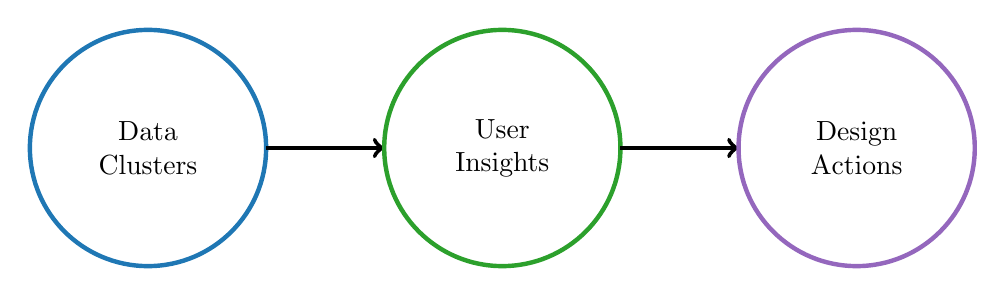
\begin{tikzpicture}[scale=1]
% Data to Empathy flow
\draw[ultra thick, mlblue] (0,0) circle (1.5);
\node[align=center] at (0,0) {Data\\Clusters};

\draw[ultra thick, ->] (1.5,0) -- (3,0);

\draw[ultra thick, mlgreen] (4.5,0) circle (1.5);
\node[align=center] at (4.5,0) {User\\Insights};

\draw[ultra thick, ->] (6,0) -- (7.5,0);

\draw[ultra thick, mlpurple] (9,0) circle (1.5);
\node[align=center] at (9,0) {Design\\Actions};
\end{tikzpicture}
\end{center}

\vspace{0.5cm}
\begin{center}
\Large\textit{``Numbers tell you what, stories tell you why''}
\end{center}
\end{frame}

% PART 4: ETHICS & PRACTICE
\part{Responsible Clustering}

% Section Divider for Part 4
\begin{frame}
\frametitle{\Large Part 4: Ethics \& Practice}
\framesubtitle{Clustering with Responsibility}

\begin{center}
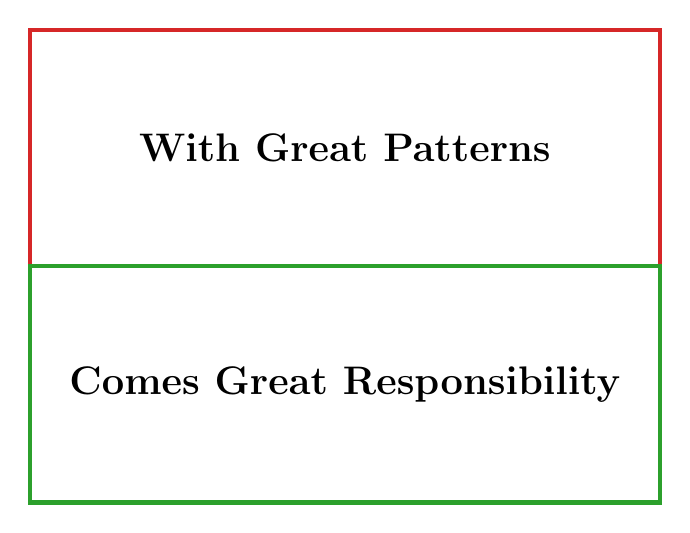
\begin{tikzpicture}[scale=1]
\node[draw, ultra thick, mlred, minimum width=8cm, minimum height=3cm] at (0,2) {};
\node[font=\Large\bfseries] at (0,2) {With Great Patterns};

\node[draw, ultra thick, mlgreen, minimum width=8cm, minimum height=3cm] at (0,-1) {};
\node[font=\Large\bfseries] at (0,-1) {Comes Great Responsibility};
\end{tikzpicture}
\end{center}
\end{frame}

% Slide 31: Case Study - Spotify
\begin{frame}
\frametitle{\Large Case Study: Spotify Discover Weekly}
\framesubtitle{30 Million Personalized Playlists Every Monday}

\begin{columns}[T]
\begin{column}{0.48\textwidth}
\textbf{\large The Challenge:}
\begin{itemize}
\item 500M+ users globally
\item 100M+ songs available
\item Diverse music tastes
\item Discovery paralysis
\end{itemize}

\vspace{0.3cm}
\textbf{\large The Solution:}
\begin{enumerate}
\item Cluster users by listening patterns
\item Find ``taste twins'' in same cluster
\item Recommend unheard songs from twins
\item Personalize 30 songs weekly
\end{enumerate}

\vspace{0.3cm}
\textbf{\large The Impact:}
\begin{itemize}
\item 40M+ weekly active users
\item 60\% listen to 10+ songs
\item 80\% save at least 1 song
\item \$1B+ value creation
\end{itemize}
\end{column}

\begin{column}{0.48\textwidth}
\begin{center}
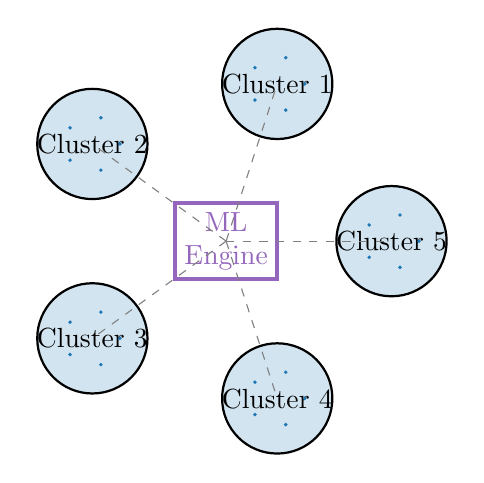
\begin{tikzpicture}[scale=0.7]
% User clusters visualization
\foreach \cluster in {1,...,5} {
    \pgfmathsetmacro{\angle}{72*\cluster}
    \pgfmathsetmacro{\xpos}{3*cos(\angle)}
    \pgfmathsetmacro{\ypos}{3*sin(\angle)}
    
    \draw[thick, fill=mlblue!20] (\xpos,\ypos) circle (1);
    \node at (\xpos,\ypos) {Cluster \cluster};
    
    % Users in cluster
    \foreach \user in {1,...,5} {
        \pgfmathsetmacro{\uangle}{360/5*\user}
        \pgfmathsetmacro{\ux}{\xpos + 0.5*cos(\uangle)}
        \pgfmathsetmacro{\uy}{\ypos + 0.5*sin(\uangle)}
        \fill[mlblue] (\ux,\uy) circle (1pt);
    }
}

% Center algorithm
\node[draw, ultra thick, mlpurple, align=center] at (0,0) {ML\\Engine};

% Connections
\foreach \cluster in {1,...,5} {
    \pgfmathsetmacro{\angle}{72*\cluster}
    \pgfmathsetmacro{\xpos}{3*cos(\angle)}
    \pgfmathsetmacro{\ypos}{3*sin(\angle)}
    \draw[dashed, gray] (0,0) -- (\xpos,\ypos);
}
\end{tikzpicture}
\end{center}

\vspace{0.3cm}
\begin{tcolorbox}[colback=mlgreen!10, colframe=mlgreen!50]
\centering\small
\textbf{Key Insight:} Users with similar taste profiles discover music through each other
\end{tcolorbox}
\end{column}
\end{columns}
\end{frame}

% Summary slide
\begin{frame}
\frametitle{\Large Week 2 Summary}
\framesubtitle{Key Takeaways}

\begin{columns}[T]
\begin{column}{0.48\textwidth}
\begin{tcolorbox}[colback=mlblue!10, colframe=mlblue!50, title=What We Learned]
\normalsize
\begin{itemize}
\item K-means finds natural user groups
\item Distance metrics matter for meaning
\item Clusters evolve into personas
\item Multiple methods for different needs
\item Ethics crucial for segmentation
\end{itemize}
\end{tcolorbox}

\vspace{0.3cm}
\begin{tcolorbox}[colback=mlgreen!10, colframe=mlgreen!50, title=Practical Skills]
\normalsize
\begin{itemize}
\item Choose optimal k with elbow method
\item Validate with silhouette analysis
\item Transform clusters to empathy maps
\item Detect and handle outliers
\item Track segment evolution
\end{itemize}
\end{tcolorbox}
\end{column}

\begin{column}{0.48\textwidth}
\begin{tcolorbox}[colback=mlorange!10, colframe=mlorange!50, title=Next Week Preview]
\normalsize
\textbf{Week 3: NLP for Emotional Context}
\begin{itemize}
\item Sentiment analysis at scale
\item BERT and transformers
\item Emotion detection
\item Sarcasm and context
\item Voice of customer analysis
\end{itemize}
\end{tcolorbox}

\vspace{0.3cm}
\begin{tcolorbox}[colback=mlpurple!10, colframe=mlpurple!50, title=Practice Exercise]
\normalsize
\textbf{This Week's Challenge:}
\begin{enumerate}
\item Take any dataset with 100+ users
\item Apply K-means with k=3,4,5
\item Use elbow method to find optimal k
\item Create personas for each cluster
\item Design one feature per persona
\end{enumerate}
\end{tcolorbox}
\end{column}
\end{columns}
\end{frame}

\end{document}